\documentclass[bachelor, och, labwork]{shiza}

\usepackage[utf8]{inputenc}
\usepackage{graphicx}

\usepackage[sort,compress]{cite}
\usepackage{amsmath}
\usepackage{amssymb}
\usepackage{amsthm}
\usepackage{fancyvrb}
\usepackage{longtable}
\usepackage{array}
\usepackage[english,russian]{babel}
\usepackage{minted}

\usepackage{tempora}


% \usepackage[colorlinks=false]{hyperref}


\newcommand{\eqdef}{\stackrel {\rm def}{=}}


\begin{document}

\title{Алгоритмы алгебры и теории чисел}

\course{4}

\group{431}

\napravlenie{10.05.01 "--- Компьютерная безопасность}


\author{Никитина Арсения Владимировича}


\satitle{доцент}
\saname{А.\,С.\,Гераськин}


\date{2022}

\maketitle

% Включение нумерации рисунков, формул и таблиц по разделам
% (по умолчанию - нумерация сквозная)
% (допускается оба вида нумерации)
%\secNumbering


\tableofcontents

\section{Задание лабораторной работы}

Осуществить проверку чисел на простоту с помощью полиномиального теста 
распознавания простоты.

\section{Теоретическая часть}

\begin{center}
    \textit{Формулировка теста Агравала-Каяла-Саксены}
\end{center}

Если существует $r\in \mathbb {Z}$ такое, что $o_{r}(n)>\log ^{2}n$ и $\forall a$ 
от $1$ до $\left\lfloor {\sqrt {\varphi (r)}}\log(n)\right\rfloor$ выполняется 
сравнение $(x+a)^{n}\equiv (x^{n}+a){\pmod {x^{r}-1,\;n}}$,
то $n$ --- либо простое число, либо степень простого числа.

$o_{r}(n)$ обозначает показатель числа $n$ по модулю $r$, $\log$ --- двоичный 
логарифм и $\varphi (\cdot )$ --- функция Эйлера.

Сравнение по двум модулям вида $a(x)\equiv b(x){\pmod {h(x),\;n}}$ для многочленов 
$a(x),\;b(x)\in \mathbb {Z} [x]$ означает, что существует $g(x)\in \mathbb {Z} [x]$
такой, что все коэффициенты многочлена $a(x)-b(x)-g(x)h(x)$ кратны $n$, где 
$\mathbb {Z} [x]$ --- кольцо многочленов от $x$ над целыми числами.

\begin{center}
    \textit{Оновная идея алгоритма}
\end{center}

Основной идеей алгоритма является обобщение малой теоремы Ферма на многочлены, 
утверждающее, что для всех $a\in \mathbb {Z} _{n}^{*}$ (где кольцо 
$\mathbb {Z} _{n}$ взято без обратных элементов по умножению и нулевого элемента)
$n\in \mathbb {N}$, $n$ --- простое тогда и только тогда, когда 
$(x+a)^{n}\equiv (x^{n}+a){\pmod {n}}$.

На проверку этого выражения требуется время, оцениваемое в $\Omega (n)$, поскольку 
в худшем случае следует оценить $n$ коэффициентов в левой части. Для сокращения 
числа коэффициентов и сложности вычислений было выбрано такое $r$, чтобы 
использовать в качестве теста на простоту выражение: $(x+a)^{n}\equiv (x^{n}+a){\pmod {x^{r}-1,\;n}}$,
которое получается делением обеих частей исходного выражения на $x^{r}-1$.

Здесь количество подлежащих проверке значений $a$ и значение $r$ уже ограничены
многочленом от $\log n$.

В этом случае вместо факторкольца $\mathbb {F} _{p}[x]/\langle x^{r}-1\rangle$ 
рассматривается поле $F=\mathbb {F} _{p}[x]/\langle h\rangle$, где $h=h(x)$ --- 
неприводимый делитель ${x^{r}-1}$ над конечным полем $\mathbb {F} _{p}$, отличный 
от $x-1$. Оценивается число многочленов этого поля, для которых выполняется сравнение:
$(x+a)^{n}\equiv (x^{n}+a){\pmod {x^{r}-1,\;n}}.$

\begin{center}
    \textit{Алгоритм теста}
\end{center}

Ввод: целое число $n>1$.

\begin{enumerate}
    \item Если $n=a^{b}$ для целых чисел $a>1$ и $b>1$, вернуть <<составное>>.
    \item Найдем наименьшее $r$, такое что $o_{r}(n)>(\log _{2}(n))^{2}$.
    \item Если $1<$НОД$(a,\;n)<n$ для некоторого $a\leqslant r$, вернуть <<составное>>.
    \item Если $n\leqslant r$, вернуть <<простое>>.
    \item Если для всех $a$ от $1$ до $\left\lfloor {\sqrt {\varphi (r)}}\log(n)\right\rfloor$ 
    верно, что $(x+a)^{n}\equiv x^{n}+a{\pmod {x^{r}-1,\;n}}$, вернуть <<простое>>.
    \item Иначе вернуть <<составное>>.
\end{enumerate}



\section{Практическая часть}
\subsection{Пример работы алгоритма}
\begin{figure}[H]
    \centering
    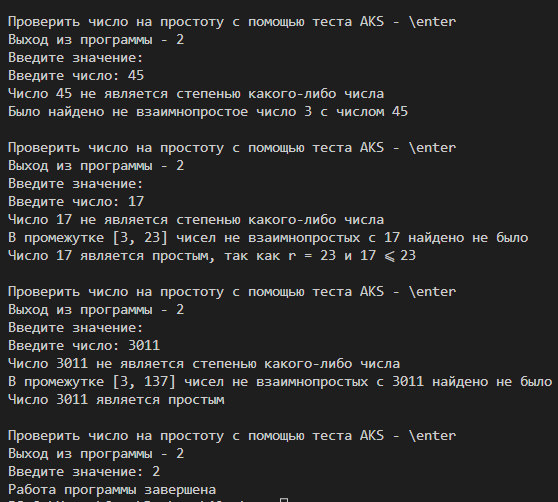
\includegraphics[width=1\textwidth]{pic1.png}
    \caption{}
\end{figure}

\setminted[python]{linenos,breaklines=true, fontsize=\small, style=bw}
    \subsection{Код программы, реализующей рассмотренный алгоритм}
        \inputminted{python}{lab8.py}

\end{document}